\documentclass[journal]{IEEEtran}

\usepackage[T1]{fontenc}
\usepackage[utf8]{inputenc}
\usepackage{amsmath,amssymb,amsfonts}
\usepackage{graphicx}
\usepackage{booktabs}
\usepackage{array}
\usepackage{url}
\usepackage{listings}
\usepackage{xcolor}
\usepackage[hidelinks]{hyperref}
\usepackage{orcidlink}
\usepackage{balance}

\graphicspath{{../figures/}}

\renewcommand{\topfraction}{0.92}
\renewcommand{\bottomfraction}{0.75}
\renewcommand{\textfraction}{0.08}
\renewcommand{\floatpagefraction}{0.80}

\lstset{
  basicstyle=\ttfamily\footnotesize, breaklines=true, columns=fullflexible,
  keepspaces=true, xleftmargin=1em, frame=single, framesep=4pt, rulecolor=\color{gray!50},
  backgroundcolor=\color{gray!6}, aboveskip=6pt, belowskip=4pt,
}

\begin{document}

\title{minehaulsim: A Deterministic Discrete-Event\\ Simulator of Mine Haulage on a\\ Constrained Road Network}

\author{Felipe~Santiba\~nez-Leal~\orcidlink{0000-0002-0150-3246}%
\thanks{F. Santiba\~nez-Leal is with the CAOS open-research programme, Santiago, Chile
(e-mail: fsantibanez@gmail.com; ORCID 0000-0002-0150-3246).}%
\thanks{Software note, 2026. Package \texttt{minehaulsim} on PyPI; source (MIT) at
\url{https://github.com/fsantibanezleal/CAOS_MINEHAUL}.}}

\markboth{Software Note, 2026}%
{Santiba\~nez-Leal: minehaulsim, a deterministic discrete-event simulator of mine haulage on a constrained road network}

\maketitle

\begin{abstract}
The productivity of an open-pit mine is set at the truck-shovel interface, where a fleet of haul trucks cycles
between shovels and dumps over a road network of ramps, junctions and single-lane segments. Simulating that
interface faithfully needs the network: travel times depend on grade, and congestion (trucks bunching behind a
slow unit on a one-way ramp) is where production is lost. Yet the open-source mine simulators use one fixed mine
layout and scalar shovel-to-dump distances with no grades and no traffic, and the tools that model the network
properly are commercial and closed. We present \texttt{minehaulsim}, a pure-Python, MIT-licensed simulator that
fills the gap: it runs mine haulage as a \emph{deterministic} discrete-event simulation on a \emph{constrained
road network} (one-way ramps, width and passing classes, single-lane direction zones, junction blocking, and a
headway-limited, first-in-first-out no-overtake rule so that bunching \emph{emerges} rather than being sampled
from a distribution), with attainable truck speed solved from rimpull and retarder envelopes against grade. A run
is a pure function of \texttt{(spec, policy, seed)} and is byte-identical across machines. Seeded parametric
generators produce a structurally different, valid open-pit or multi-level underground mine per seed, and every
run exports interoperable cycle logs. We demonstrate the simulator on a generated pit: production rises with the
fleet and then \emph{saturates} (from $243$ to $4{,}800$ tonnes per hour as the fleet grows to $22$ trucks, the
truck busy fraction falling from $1.0$ to $0.70$ as trucks begin to queue), the constrained network costs a
$6$--$10\%$ production loss over free-flow in the fleet-matched region, and the dispatch policy matters
(shortest-queue $3{,}766$ vs nearest-shovel $2{,}874$ tonnes per hour at a matched fleet). We are explicit about
what the model is and is not; every number and figure regenerates from the committed run.
\end{abstract}

\begin{IEEEkeywords}
Discrete-event simulation, open-pit mining, truck-shovel haulage, road network, dispatch policy, match factor,
determinism, reproducible software.
\end{IEEEkeywords}

\section{Introduction}

\IEEEPARstart{O}{pen-pit} mine production is governed by the truck-shovel haulage cycle: trucks load at shovels,
haul loaded up the ramp to a crusher or waste dump, dump, and return empty to a shovel chosen by a dispatch
policy~\cite{alarie,newman}. Sizing the fleet, choosing the dispatch policy, and understanding where production
is lost are classic operations-research questions~\cite{burt}, and the tool for them is
simulation~\cite{robinson}. The fidelity of that simulation hinges on one thing: the road network. Travel time is
not a constant between a shovel and a dump; it depends on the grade the loaded truck climbs and on congestion,
the bunching that forms when a fast truck catches a slow one on a one-way ramp it cannot pass. A simulator that
represents haul roads as scalar distances cannot see either effect, and it is exactly there that a real operation
gains or loses tonnes.

The open-source tooling does not close this gap. The available simulators model a single fixed mine layout with
scalar shovel-to-dump distance matrices, no grades or rimpull, and no traffic constraints; the recent
\texttt{OpenMines} environment~\cite{openmines}, for instance, is built for dispatch-policy research on an
abstract road graph rather than a constrained physical network. The tools that do model the network correctly
(HAULSIM, TALPAC-3D, SimMine) are commercial and closed. A researcher who wants to study dispatch on a realistic
constrained network, or a downstream tool that needs structure-real haulage scenarios, has nothing open to build
on.

\texttt{minehaulsim} is that open tool. It is a pure-Python, MIT-licensed package that simulates open-pit and
underground mine haulage as a deterministic discrete-event process on a constrained road network. Its design
commitments are: (i) the \emph{network is first-class}, so travel times come from route kinematics on a directed
multigraph with one-way ramps, passing classes, single-lane zones, junction blocking and headway capacity, and
congestion emerges from a no-overtake rule rather than being sampled; (ii) attainable speed is \emph{solved from
grade} via rimpull and retarder force envelopes; (iii) a run is \emph{deterministic}, a pure function of
\texttt{(spec, policy, seed)}, byte-identical across machines; and (iv) mines are \emph{generated}, a
structurally different valid mine per seed rather than one layout reused. This note describes those commitments
and demonstrates them on a generated pit, with an explicit statement of what the model does and does not
represent.

\section{Statement of Need}\label{sec:need}

The users are researchers and tool-builders who need realistic, reproducible mine-haulage scenarios and cannot
use the closed commercial simulators. A dispatch-policy study needs a constrained network on which congestion is
real, not a scalar-distance abstraction on which every policy looks the same. A downstream planning or dispatch
tool (the consumer this package was built for) needs structure-real haulage samples with cycle logs it can
ingest, and a course needs mines a student can generate and simulate on a laptop. The deterministic core matters
for all three: a byte-identical run is a testable, citable object, so a result can be reproduced exactly and a
regression caught precisely. \texttt{minehaulsim} provides this as a small pure-Python package under a permissive
license, with the network, the grade-based kinematics, the emergent congestion, the seeded generators and the
interoperable outputs that the open alternatives lack.

\section{The Constrained Network and Speed by Grade}\label{sec:network}

\begin{figure}[!t]
\centering
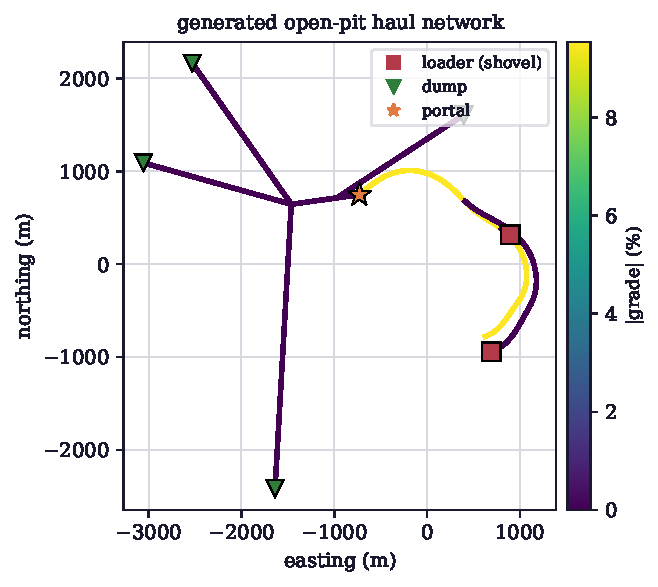
\includegraphics[width=0.86\columnwidth]{fig-network.pdf}
\caption{A generated open-pit haul network (one \texttt{generate\_open\_pit} call). The road polylines are
coloured by grade: the steep spiral access ramp descending into the pit to the two shovels (high grade) and the
flatter external haul roads fanning out to the four dumps. Travel time is computed on this network, not from a
scalar distance.}
\label{fig:network}
\end{figure}

A haul network is a directed multigraph whose segments are real road polylines carrying a length, a grade, a
width/passing class, a speed limit, a rolling-resistance and optional one-way and single-lane-zone attributes
(Fig.~\ref{fig:network}). On this network the attainable speed of a truck is not a constant but is solved from
its tractive envelope, in the TALPAC/FPC tradition~\cite{burt}: the force a truck can deliver at speed $v$ is
\begin{equation}
F(v) \;=\; \min\!\left(F_{\text{traction}},\; \frac{\eta\,P}{v}\right),
\end{equation}
the smaller of a traction limit and the power-limited pull ($P$ engine power, $\eta$ drivetrain efficiency), and
the steady speed on a segment is where this pull balances the grade and rolling resistance for the truck's gross
vehicle weight; a retarder envelope caps the descending (empty, down-grade) speed. Travel time on a route is the
integral of these segment kinematics, so a loaded truck climbing a $9\%$ ramp is correctly slower than the same
truck returning empty. Congestion is layered on top: each segment has a headway-limited capacity and a
first-in-first-out no-overtake rule, single-lane zones arbitrate opposing traffic through passing bays, and
junctions block conflicting movements, so when a fast truck catches a slow one it must follow, and \emph{bunching
emerges} from the network dynamics rather than being drawn from a delay distribution.

\section{The Deterministic Discrete-Event Core}\label{sec:des}

\begin{figure*}[!t]
\centering
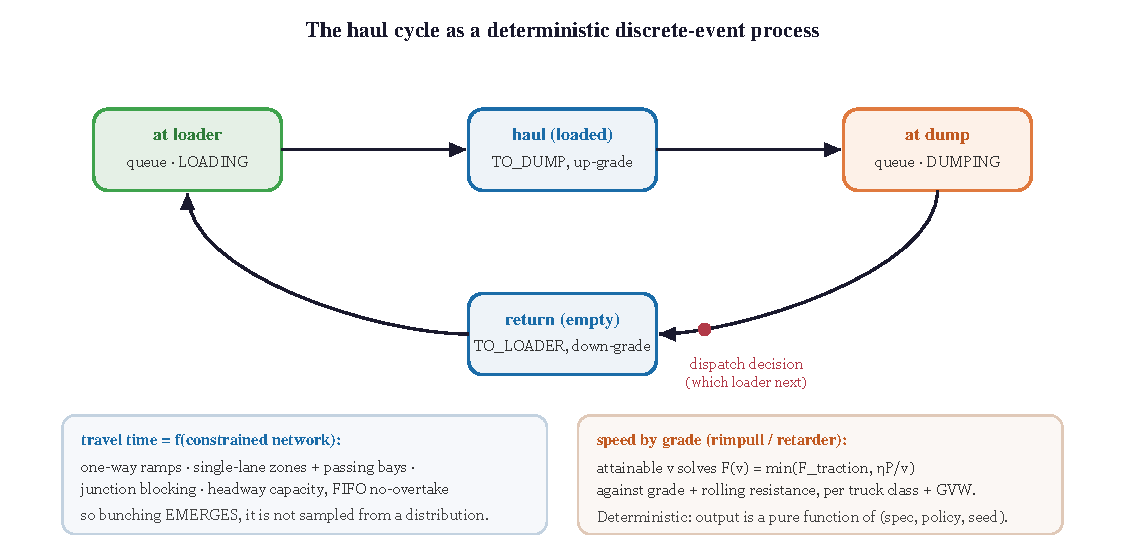
\includegraphics[width=0.99\textwidth]{fig-cycle.pdf}
\caption{The haul cycle as a deterministic discrete-event process. A truck cycles queue--load, haul loaded
(up-grade), queue--dump, and return empty (down-grade), with a dispatch decision on each return choosing the next
shovel. Travel times come from the constrained network (left), so congestion emerges rather than being sampled;
attainable speed is solved from the rimpull/retarder envelope against grade (right). The whole run is a pure
function of \texttt{(spec, policy, seed)}.}
\label{fig:cycle}
\end{figure*}

The engine is a hand-rolled discrete-event simulator (no third-party framework), processing timestamped events in
order. Each truck repeats the cycle of Fig.~\ref{fig:cycle}: it travels to a shovel, queues, loads (payload and
load time from named random streams), hauls loaded to a dump, queues, dumps, and on completion a
\emph{dispatch policy} chooses its next shovel, after which it returns empty and the cycle repeats. Loaders at
depleted or closed faces refuse service, and every completed load debits the block model so simulated tonnes and
planned depletion are the same number by construction. The single most important property is determinism: all
randomness is drawn from named, seeded streams (payload, load time, dump time, policy tie-breaks), so a run is a
pure function of its \texttt{(spec, policy, seed)} and is byte-identical across operating systems and sessions.
This makes a simulated shift a reproducible, testable object rather than a Monte-Carlo sample that changes every
time. The dispatch policy is a pluggable hook; the package ships transparent baselines (fixed assignment,
nearest shovel, shortest queue, least saturation) for research comparison, deliberately not a commercial
fleet-management optimiser.

\section{Demonstration}\label{sec:results}

\begin{figure}[!t]
\centering
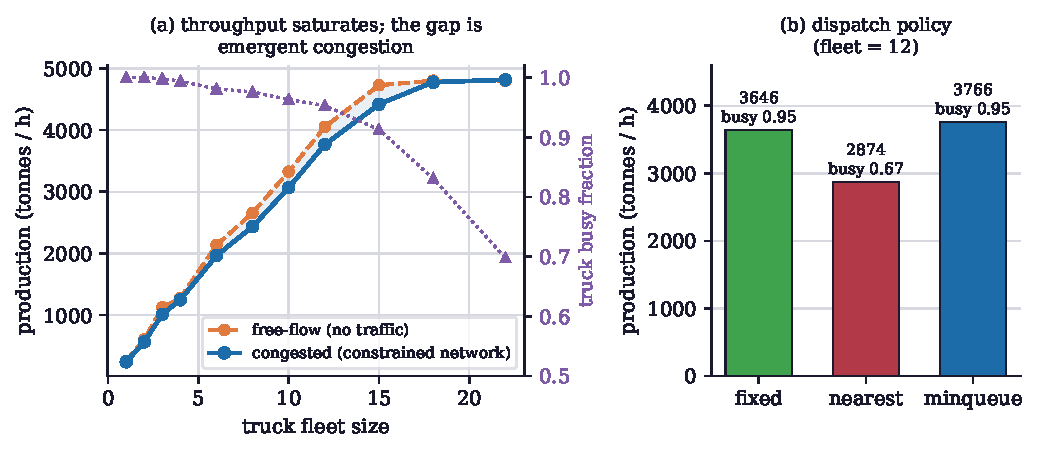
\includegraphics[width=0.99\columnwidth]{fig-throughput.pdf}
\caption{The simulator on one generated pit, six-hour shifts, deterministic. \textbf{(a)} Production rises with
the truck fleet and saturates as the shovels become the bottleneck; the truck busy fraction (right axis) falls
from $1.0$ to $0.70$ as added trucks begin to queue. The gap between the free-flow (no-traffic) and congested
(constrained-network) curves is the emergent congestion, a $6$--$10\%$ production loss in the fleet-matched
region. \textbf{(b)} At a matched fleet of $12$ trucks the dispatch policy matters: shortest-queue and fixed keep
the fleet busy ($3{,}766$ and $3{,}646$ t/h), while greedy nearest-shovel overloads one shovel and idles trucks
($2{,}874$ t/h, busy $0.67$).}
\label{fig:throughput}
\end{figure}

To show the simulator produces the phenomena a haulage study cares about, we run it on a single generated pit
(fixed geometry, seed 42) over six-hour shifts, sweeping the truck fleet and comparing dispatch policies
(Fig.~\ref{fig:throughput}); every run is deterministic. Three results emerge, none of them put in by hand.
\emph{Production saturates}: it climbs from $243$ tonnes per hour with one truck to about $4{,}800$ with $22$,
but the marginal truck earns steadily less as the shovels saturate, and the truck busy fraction falls from $1.0$
to $0.70$, the classical match-factor tradeoff. \emph{Congestion is real}: the constrained-network run trails the
free-flow run by $6$--$10\%$ through the fleet-matched region, a loss produced purely by the no-overtake network
dynamics; the two curves converge only once the shovel bottleneck dominates. \emph{Dispatch matters}: at a
matched fleet of $12$ trucks, shortest-queue dispatch delivers $3{,}766$ t/h and fixed assignment $3{,}646$,
while greedy nearest-shovel drops to $2{,}874$ (busy fraction $0.67$) because it piles trucks onto the closest
shovel and starves the other. These are the questions a mine planner asks, answered on a network where the
answers depend on the roads.

\section{Generators, Outputs and Availability}\label{sec:arch}

\texttt{minehaulsim} generates mines rather than reusing a layout: seeded parametric generators build open pits
(perturbed-superellipse rims, three ramp topologies, phases, multiple shovels and dumps) and multi-level
underground mines (declines with passing bays, drift zones, ore passes, shaft bins), each gated by named validity
checks, so every seed yields a structurally different valid mine. Every run exports interoperable artifacts: a
\texttt{cyclelog/v1} CSV event log (load/haul/dump/return), a provenance JSON, a per-truck position trace, and a
topography export for 3D viewers. The core is NumPy-only (visualisation is an opt-in extra that the core never
imports), so it installs and runs anywhere Python does. The package is deterministic, extensively unit-tested
(the network, the kinematics, the DES, the generators, the planning coupling, the failure processes with a
performance floor, the output contracts), MIT-licensed, and consumed by a downstream dispatch tool. A generated
mine is simulated in a few lines:

\begin{lstlisting}[language=Python]
from minehaulsim import generate_open_pit
from minehaulsim.des.dispatch import MinQueuePolicy
spec = generate_open_pit(seed=42)
res  = spec.run(policy=MinQueuePolicy(), seed=7, until_s=6*3600)
res.tonnes, res.cycles, res.truck_wait_s
\end{lstlisting}

Source and the reproducible demonstration of this note are at
\url{https://github.com/fsantibanezleal/CAOS_MINEHAUL}.

\section{What It Is and Is Not}\label{sec:limits}

The scope is stated honestly, and the package ships an explicit ``what it is and is not'' page. Equipment curves
are class-representative envelopes generated from first principles around public spec-sheet magnitudes, not a
manufacturer's performance table; cycle times behave like the machine class but must not be used for procurement.
The material is a single homogeneous tonnes stream: there is no ore grade, blending, dilution or stockpile
rehandle, and no fuel, tyre or emissions accounting in this version. Generated mines are synthetic,
\emph{structure-real at best and always labelled} in the provenance; nothing here predicts a specific operation
without calibration to its data. The dispatch policies are transparent research baselines, not a commercial
fleet-management system; the optimisation tier lives in consumers, not here. And the current version carries
stated simplifications: truck breakdowns materialise at cycle boundaries, surface roads are modelled flat between
graded ramps, and the underground shaft hoist is a continuous drain rather than a skip cycle. None of this is
hidden; the honesty page is the first thing the documentation asks a user to read.

\section{Conclusion}

\texttt{minehaulsim} gives the open-source community what it lacked: a deterministic discrete-event simulator of
mine haulage on a genuinely constrained road network, where travel time follows grade, congestion emerges from
no-overtake network dynamics, mines are generated rather than reused, and a run is a byte-identical function of
its inputs. On a generated pit it reproduces the phenomena a haulage study needs, production saturation, an
emergent congestion loss, and a dispatch-policy gap, on a network where those effects are real rather than
assumed. The value is a permissively-licensed, reproducible foundation for haulage and dispatch research, and for
the downstream tools that need structure-real mine scenarios.

\appendices
\section{Reproduction}\label{app:repro}

The demonstration is \texttt{manuscripts/haulage-des/figures/haulage\_sim.py}: it generates the seed-42 pit,
sweeps the truck fleet under shortest-queue dispatch in both congested and free-flow modes, compares the dispatch
policies at a matched fleet, and exports the road network, writing \texttt{data/haulage\_sim.json} and
\texttt{data/network.json}. The figure script reads those artifacts; the haul-cycle schematic is a hand-authored
theme-aware drawing. Because every run is a pure function of \texttt{(spec, policy, seed)}, re-running reproduces
every number in Section~\ref{sec:results} and Figs.~\ref{fig:network}--\ref{fig:throughput} exactly.

\balance

\begin{thebibliography}{00}

\bibitem{alarie} S.~Alarie and M.~Gamache, ``Overview of solution strategies used in truck dispatching systems
for open pit mines,'' \emph{International Journal of Surface Mining, Reclamation and Environment}, vol.~16,
no.~1, pp.~59--76, 2002. doi:10.1076/ijsm.16.1.59.3408.

\bibitem{newman} A.~M. Newman, E.~Rubio, R.~Caro, A.~Weintraub, and K.~Eurek, ``A review of operations research
in mine planning,'' \emph{Interfaces}, vol.~40, no.~3, pp.~222--245, 2010. doi:10.1287/inte.1090.0492.

\bibitem{burt} C.~N. Burt and L.~Caccetta, ``Equipment selection for surface mining: A review,''
\emph{Interfaces}, vol.~44, no.~2, pp.~143--162, 2014. doi:10.1287/inte.2013.0732.

\bibitem{robinson} S.~Robinson, ``Conceptual modeling for simulation,'' in \emph{Proc. 2013 Winter Simulation
Conference (WSC)}, 2013, pp.~377--388. doi:10.1109/WSC.2013.6721435.

\bibitem{morgan} W.~C. Morgan and L.~L. Peterson, ``Determining shovel-truck productivity,'' \emph{Mining
Engineering}, vol.~20, pp.~76--80, 1968.

\bibitem{openmines} S.~Meng \emph{et al.}, ``OpenMines: A light and comprehensive mining simulation environment
for truck dispatching,'' 2024. arXiv:2404.00622.

\bibitem{cat} Caterpillar Inc., \emph{Caterpillar Performance Handbook}. Peoria, IL: Caterpillar (rimpull,
retarder and rolling-resistance reference for haul-truck speed-by-grade).

\end{thebibliography}

\end{document}
